\begin{figure}[!htb]
    \centering
    \begin{subfigure}[b]{0.49\textwidth}
        \centering
        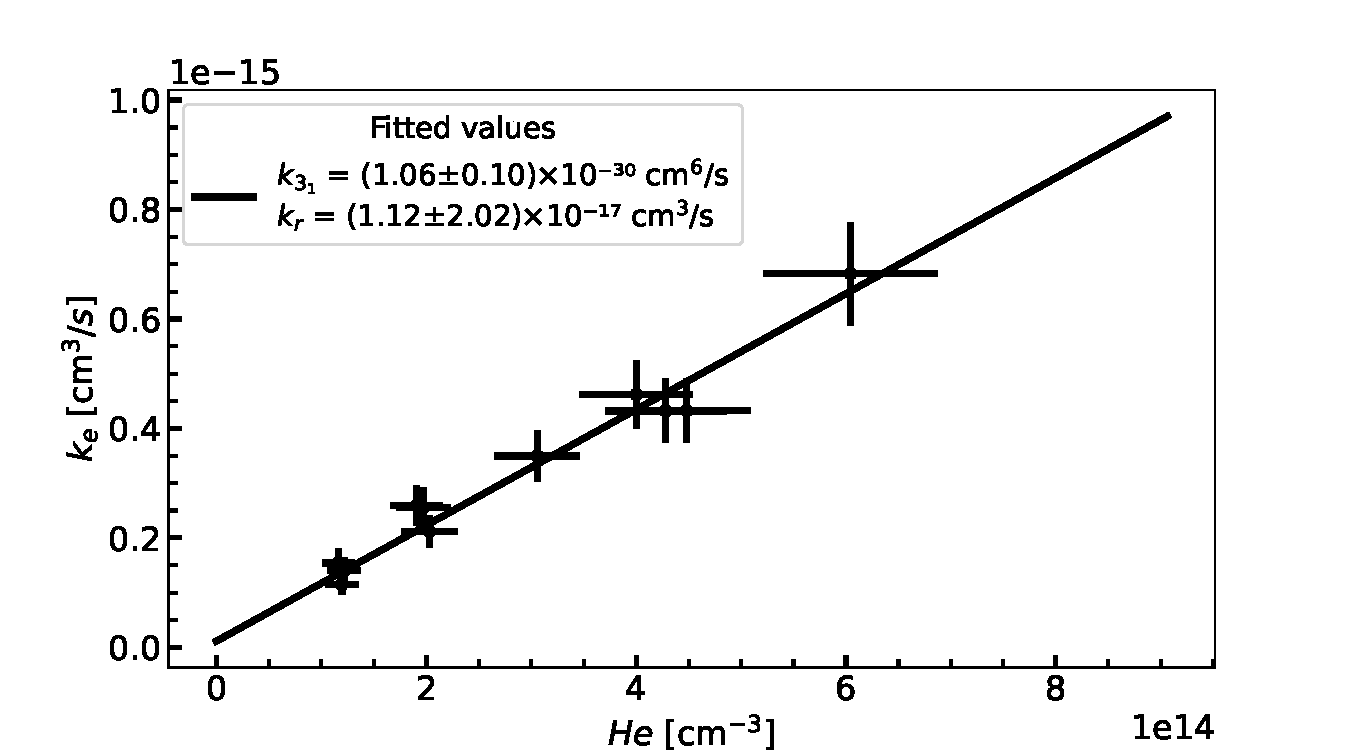
\includegraphics[width=1\textwidth]{figures/measurements/kinetics/functionOf_nHe/off_4.8K_k31_effective_rate_constants.pdf}
        
        \caption{}
        \label{fig:off:effective-rate-constants}
    \end{subfigure}
    \hfill
    \begin{subfigure}[b]{0.49\textwidth}
        \centering
        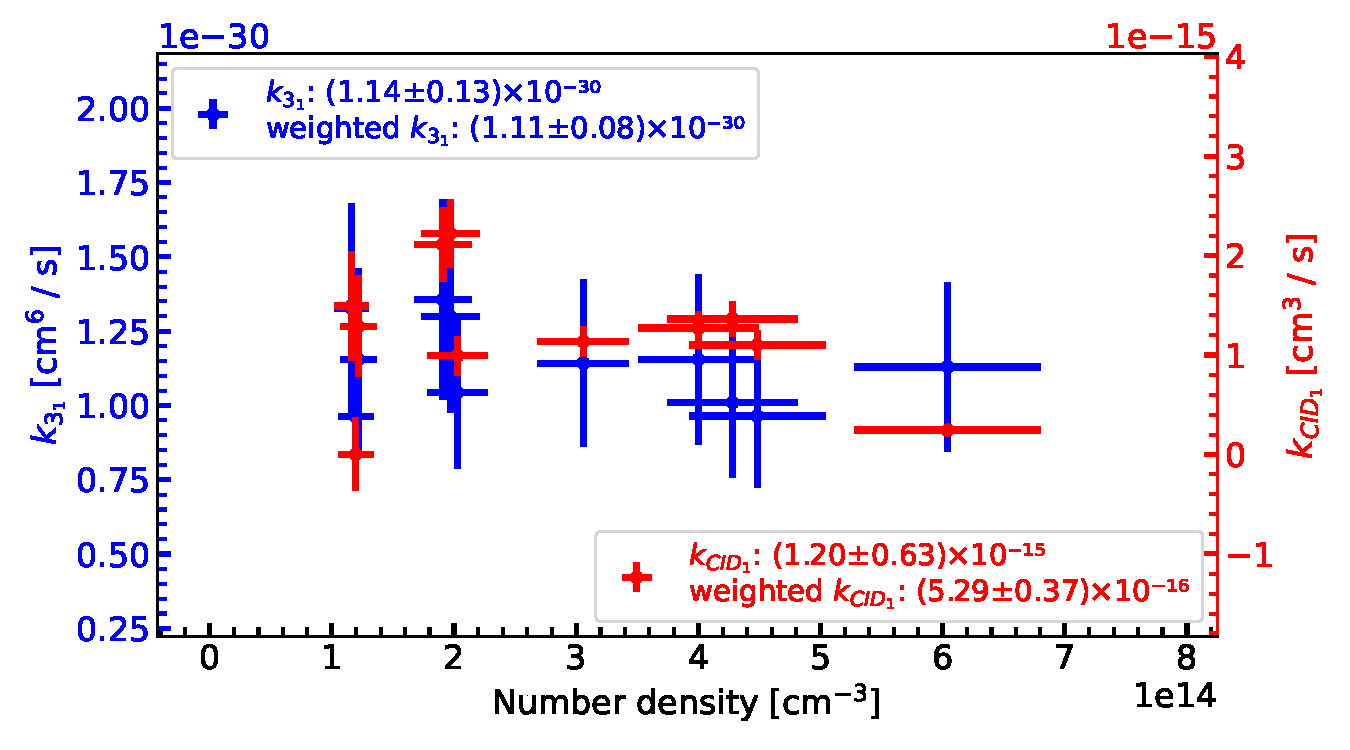
\includegraphics[width=1\textwidth]{figures/measurements/kinetics/functionOf_nHe/off_4.8K_k3_kCID_1_as_functionOfnHe.pdf}
        \caption{}
        \label{fig:off:rate-constants}
    \end{subfigure}
    
    \caption{The effective binary rate constant ($k_e$), the ternary association (\textcolor{blue}{$k_{3_1}$}) and collision-induced dissociation (\textcolor{red}{$k_{CID_1}$}) rate constants are plotted as a function of helium number density. (a) The effective binary rate constant ($k_e$) is plotted as a function of number density to derive $k_{3_1}$ (ternary association) and $k_r$ (radiative) rate constants. The solid line indicates the linear fit where the slope and intercept correspond to $k_3$ and $k_r$, respectively. (b) shows the $k_{3_1}$ as a function of number density under $k_3[He] \gg k_r$ assumption (see text). The weighted mean values are shown in the legend box.}

\end{figure}
